\documentclass[12pt,a4paper]{report}

% Packages
\usepackage{graphicx}
\usepackage{amsmath}
\usepackage{hyperref}
\usepackage{setspace}
\usepackage{float}
\usepackage{geometry}
\usepackage{enumitem}
\usepackage{circuitikz}
\usepackage{tikz}
\usepackage{booktabs}

% Title and Author
\title{\LARGE \textbf{Bode Plot Analysis of 1-Stage, 2-Stage, and 3-Stage RC Low-Pass Filters}}
\author{}
\date{\large On: \today}

% Begin Document
\begin{document}

% Title Page
\begin{titlepage}
    \centering
    \vspace*{1cm}
    { 
\includegraphics[width=6cm]{figs/logo.jpg}}\\[1cm]
    {\LARGE \textbf{EXPERIMENT 3}}\\[1cm]
    \textbf{Instructor: }{Prof. Gajendranath Chowdary}\\[1cm]
    \textbf{Written By:}\\{RONGALI CHARAN - EE24BTECH11052\\ ANKIT JAINAR - EE24BTECH11004}\\[1cm] \date{\large Date Last Edited: \today}
\end{titlepage}

% Abstract
\chapter*{Abstract}
\addcontentsline{toc}{chapter}{Abstract}
This report presents a comprehensive analysis of the Bode plot of magnitude and phase response for 1-stage, 2-stage, and 3-stage RC low-pass filters. The study includes theoretical derivations, mathematical modeling, and experimental validation through oscilloscope measurements. 

The Bode plot provides insight into the frequency response characteristics of filters, showcasing the attenuation and phase shift as a function of input frequency. This analysis is crucial for designing effective signal conditioning circuits in electronic applications.

The effects of cascading multiple RC stages on frequency response are explored. Practical implementation details, including breadboard setup, expected readings, and component tolerances, are thoroughly discussed. The study aims to bridge theoretical concepts with real-world circuit behavior by comparing calculated and observed responses, emphasizing the importance of low-pass filtering in signal processing applications.

% Table of Contents
\tableofcontents

% List of Figures
\listoffigures

\chapter{One-Stage RC Low-Pass Filter Setup}
\section{Single-Stage RC Low-Pass Filter Connection}
A single-stage RC low-pass filter consists of a resistor and capacitor connected in series, where the output is taken across the capacitor. The circuit is configured as follows:
\begin{itemize}
    \item Resistor: \( R = 10k\Omega \)
    \item Capacitor: \( C = 0.01\mu F \)
    \item Function generator providing sinusoidal input
    \item Oscilloscope for measuring voltage response
\end{itemize}

\subsection*{Breadboard Connections}
\begin{enumerate}
    \item Place the resistor and capacitor in series on the breadboard.
    \item Connect the input signal to one end of the resistor.
    \item Connect the other end of the resistor to one terminal of the capacitor.
    \item Connect the remaining terminal of the capacitor to the ground.
    \item Attach oscilloscope probes across the capacitor to observe the output.
\end{enumerate}

\subsection{Circuit Diagram}
\begin{figure}[H]
    \centering
    \begin{circuitikz}
        \draw (0,0) to[sinusoidal voltage source, l=$V_{in}$] (0,2)
              to[R, l=$R$] (3,2)
              to[C, l=$C$] (3,0)
              -- (0,0);
        \draw (3,2) -- (4,2) ;
        \draw (3,2) to[short, -*] (4,2);
        \draw (3,0) -- (4,0) node[right] at (4,1) {{$V_{out}$}};
        \draw (3,0) to[short, -*] (4,0);
    \end{circuitikz}
    \caption{1-Stage RC Low-Pass Filter}
\end{figure}


\subsection{Theoritical equations}
The expected output voltage is given by:
\begin{align}
 H_1(\omega) &= \frac{1}{1 + j\omega R C} \\
 |H_1(\omega)| &= \frac{1}{\sqrt{1 + (\omega R C)^2}}\\
 \theta_1(\omega) &= -\tan^{-1}(\omega R C) 
\end{align}
The magnitude response in decibels (dB) is given by:

\begin{align}
20 \log_{10} |H(\omega)|
\end{align}
The phase response in degrees is:

\begin{align}
\theta(\omega) \times \frac{180}{\pi}
\end{align}

where \( H(j\omega) \) is the transfer function.
\newpage
\section*{1-Stage RC Low-Pass Filter Analysis}
\begin{table}[h]
    \centering
    \begin{tabular}{r c c c c}
        \toprule
        $f$(Hz) & $V_{in}$(V) & $V_{out}$ Theoretical(V) & $V_{out}$ Experimental(V) & $\Delta t$\\
        \midrule
        100  & 2.161 & 2.157 & 2.081 & -98.000$\mu s$\\
        500  & 2.161 & 2.062 & 1.921 & -94.892$\mu s$\\
        1000 & 2.161 & 1.830 & 1.681 & -87.783$\mu s$\\
        1590 & 2.161 & 1.529 & 1.441 & -76.068$\mu s$\\
        3000 & 2.161 & 1.013 & 1.041 & -55.457$\mu s$\\
        5000 & 2.161 & 0.655 & 0.700 & -41.191$\mu s$\\
        10000 & 2.161 & 0.340 & 0.384 & -24.488$\mu s$\\
        \bottomrule
    \end{tabular}
    \caption{1-Stage RC Low-Pass Filter Analysis}
\end{table}
\begin{itemize}
    \item The values of $\Delta t$ are taken by measuring difference between peaks.
    \item The signs of $\Delta t$ were placed according to the theory for correct phase plot.
\end{itemize}
\subsection{Bode Plot}
\begin{figure}[H] % H forces the figure to be placed exactly here
    \centering
    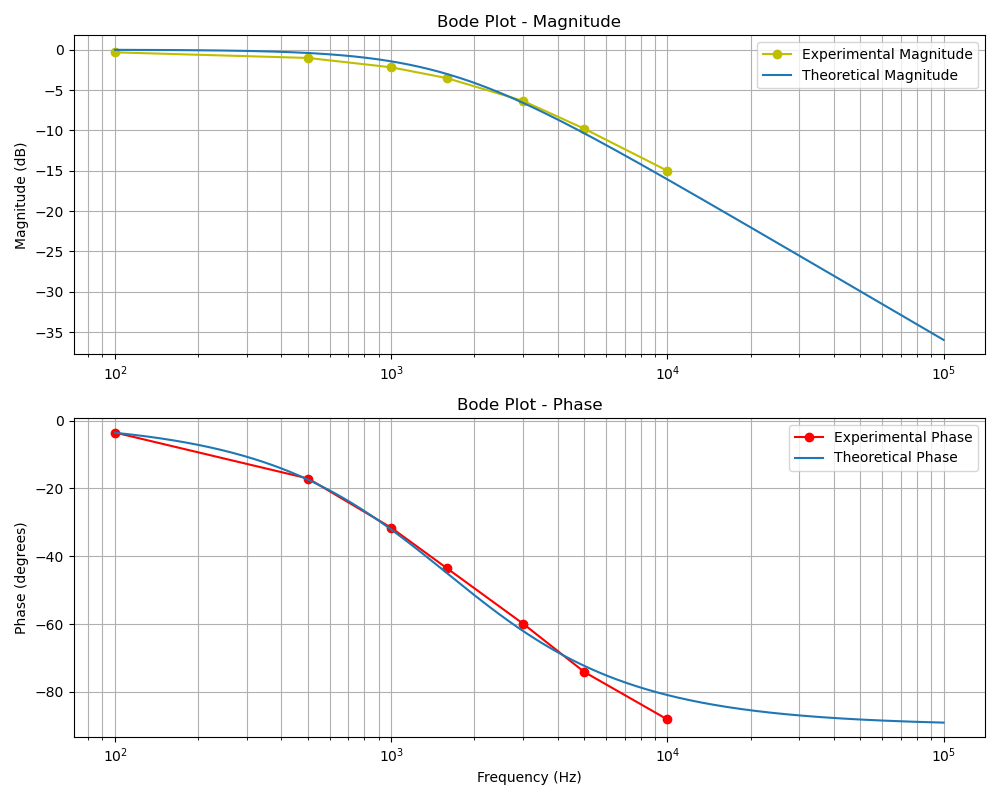
\includegraphics[width=\textwidth]{figs/1phase.png}\\% Replace "1.jpg" with your actual image filename
    
    
    \caption{1 stage bode plot}
    \label{fig:bode plot}
\end{figure}
\begin{figure}
    \centering
    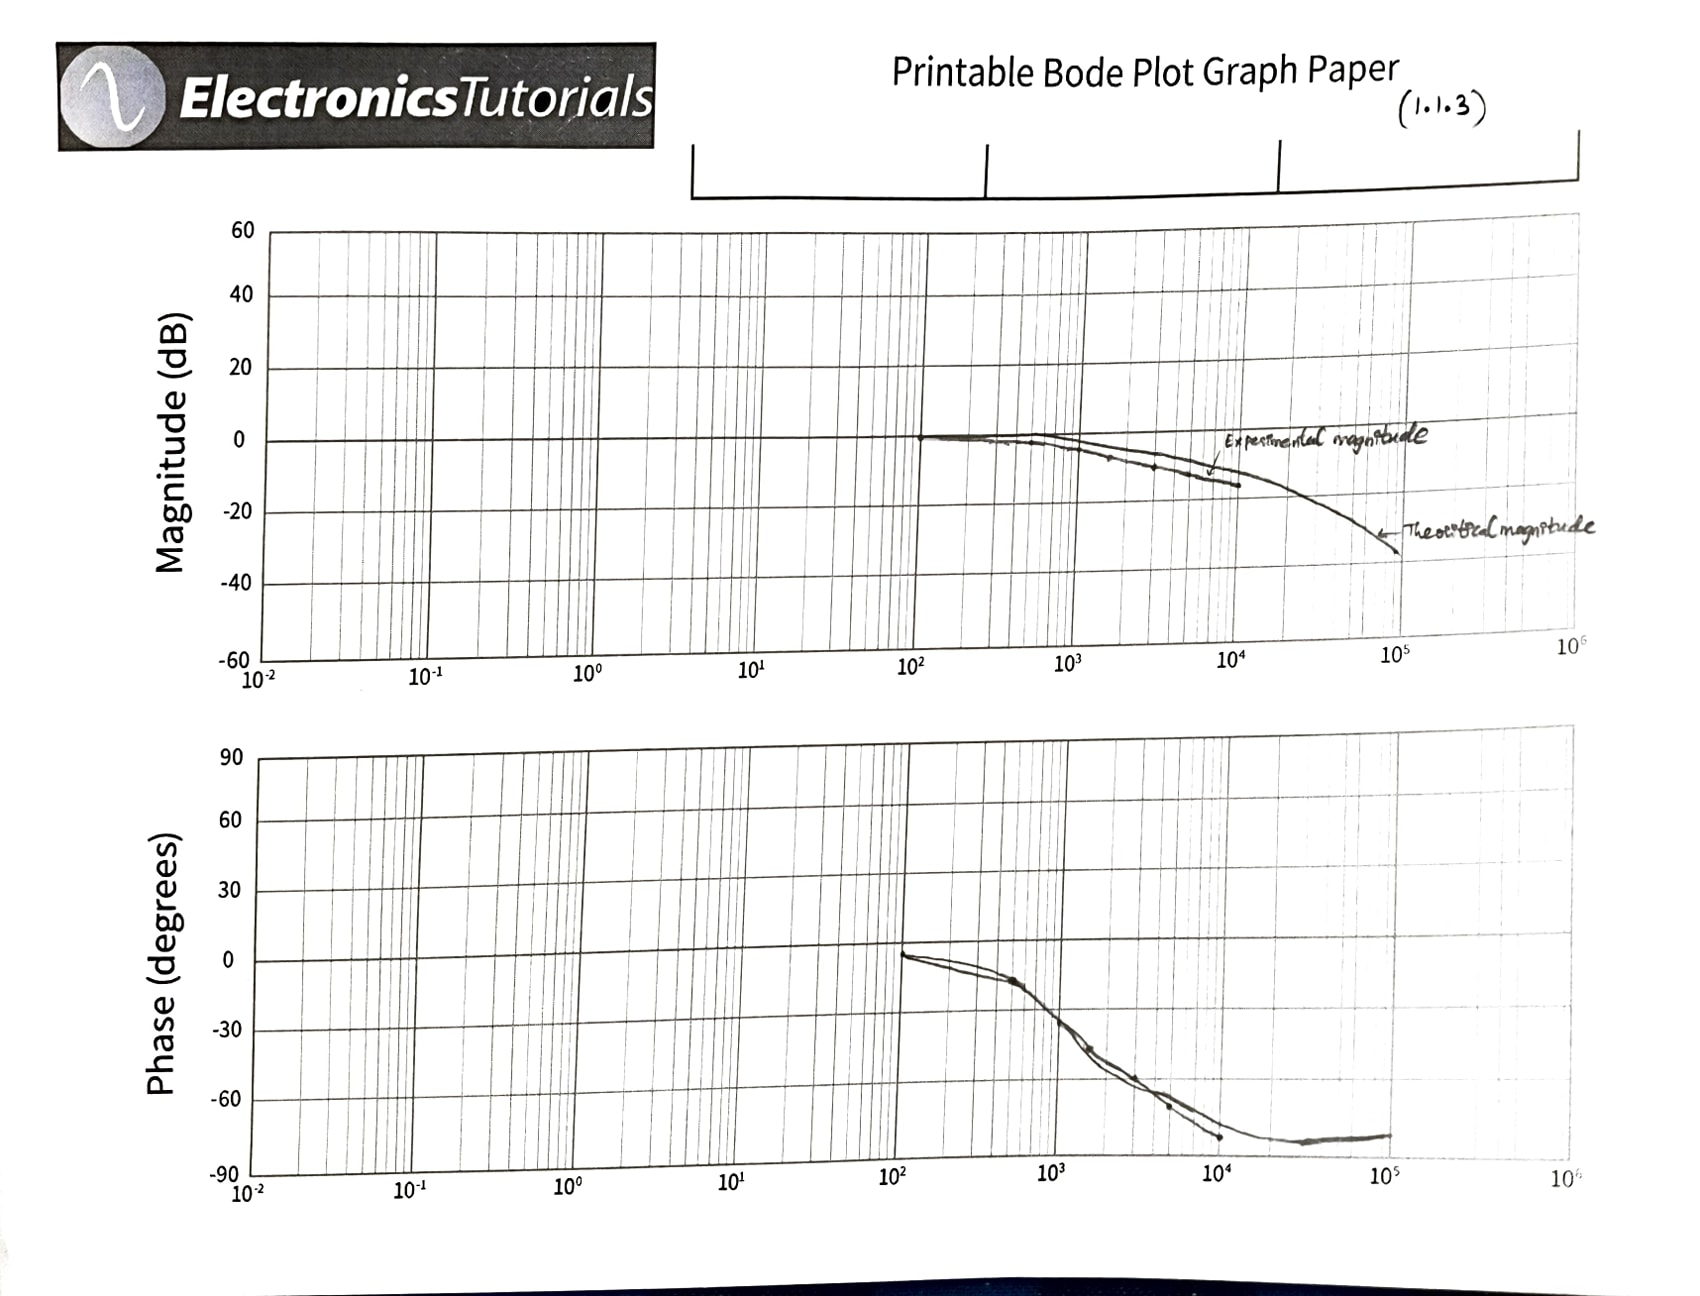
\includegraphics[width=\linewidth]{figs/1draw.jpg}
    
    \label{fig:enter-label}
\end{figure}
At low frequencies, the output approximates the input signal. As frequency increases, the magnitude decreases at a rate of \(-20\) dB/decade beyond the cutoff frequency \( f_c = \frac{1}{2\pi RC} \).

\chapter{Two-Stage RC Low-Pass Filter Setup}
\section{Two-Stage RC Low-Pass Filter Connection}
When two RC stages are cascaded, the attenuation increases, resulting in sharper roll-off characteristics. The addition of another RC network significantly enhances the filtering effect.
Make circuit connection as shown

\subsection{Circuit Diagram}
\begin{figure}[h]
    \centering
    \begin{circuitikz}
        \draw (0,0) to[sinusoidal voltage source, l=$V_{in}$] (0,2)
              to[R, l=$R$] (3,2)
              to[C, l=$C$] (3,0)
              -- (0,0);
        \draw (3,2) to[R, l=$R$] (6,2)
              to[C, l=$C$] (6,0)
              -- (3,0);
        \draw (6,2) to[short, -*] (7,2) node[right] at (7,1){$V_{out}$};
        \draw (6,0) to[short, -*] (7,0)  ;
    \end{circuitikz}
    \caption{2-Stage RC Low-Pass Filter}
\end{figure}
\subsection{Theoritical equations}
The expected output voltage is given by:
\begin{align}
 H_2(\omega) &= \frac{1}{1 + (j\omega R C)^2 + 3 j\omega R C} \\
 |H_2(\omega)| &= \frac{1}{\sqrt{(1 - (\omega R C)^2)^2 + (3\omega R C)^2}}\\
 \theta_2(\omega) &= -\tan^{-1} \left( \frac{3\omega R C}{1 - (\omega R C)^2} \right)
\end{align}
The magnitude response in decibels (dB) is given by:

\begin{align}
20 \log_{10} |H(\omega)|
\end{align}
The phase response in degrees is:

\begin{align}
\theta(\omega) \times \frac{180}{\pi}
\end{align}

where \( H(j\omega) \) is the transfer function.
\section*{2-Stage RC Low-Pass Filter Analysis}
\begin{table}[h]
    \centering
    \begin{tabular}{r c c c c}
        \toprule
        $f$(Hz) & $V_{in}$(V) & $V_{out}$ Theoretical(V) & $V_{out}$ Experimental(V) &  $\Delta t$\\
        \midrule
        100  & 2.161 & 2.132 & 2.052 & -303.240$\mu s$\\
        500  & 2.161 & 1.657 & 1.498 & -262.410$\mu s$\\
        1000 & 2.161 & 1.092 & 1.041 & -203.920$\mu s$\\
        1590 & 2.161 & 0.721 & 0.687 & -162.170$\mu s$\\
        3000 & 2.161 & 0.348 & 0.362 & 62.952$\mu s$\\
        5000 & 2.161 & 0.167 & 0.184 & 26.612$\mu s$\\
        10000 & 2.161 & 0.050 & 0.071 & 7.894$\mu s$\\
        \bottomrule
    \end{tabular}
    \caption{2-Stage RC Low-Pass Filter Analysis}
\end{table}
\begin{itemize}
    \item The values of $\Delta t$ are taken by measuring difference between peaks.
    \item The signs of $\Delta t$ were placed according to the theory for correct phase plot.
\end{itemize}
\subsection{Bode Plot}
\begin{figure}[H] % H forces the figure to be placed exactly here
    \centering
    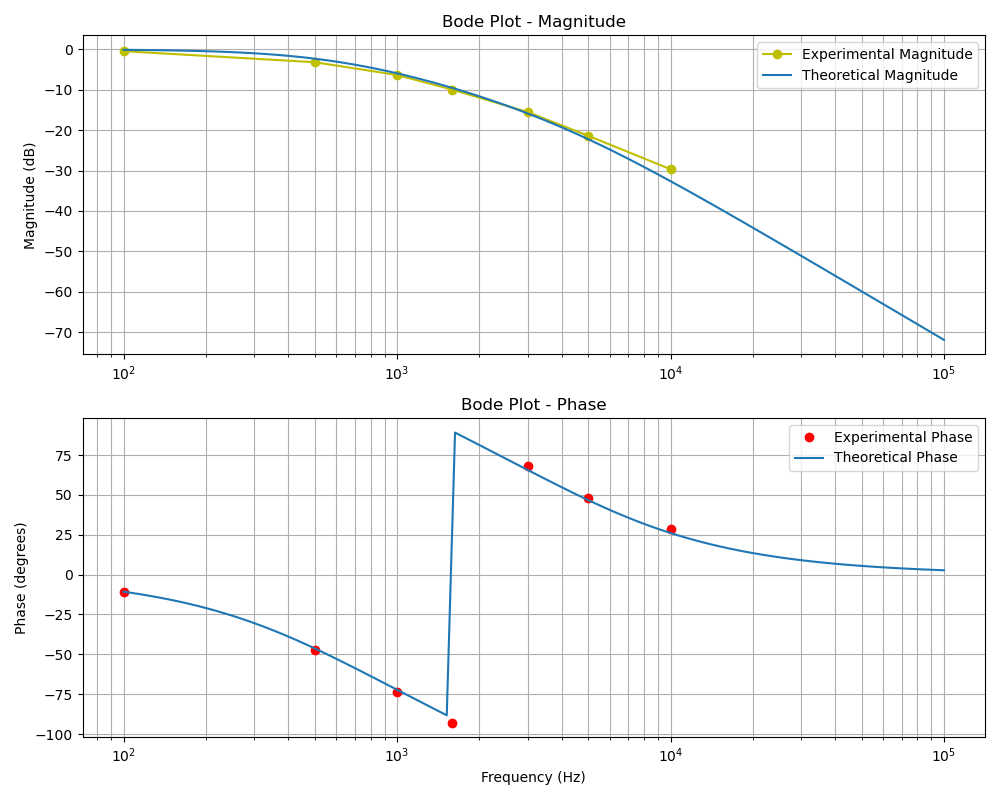
\includegraphics[width=\textwidth]{figs/2phase.png} % Replace "1.jpg" with your actual image filename
    
    \caption{2 stage bode plot}
    \label{fig:bode plot}
\end{figure}
\begin{figure}
    \centering
    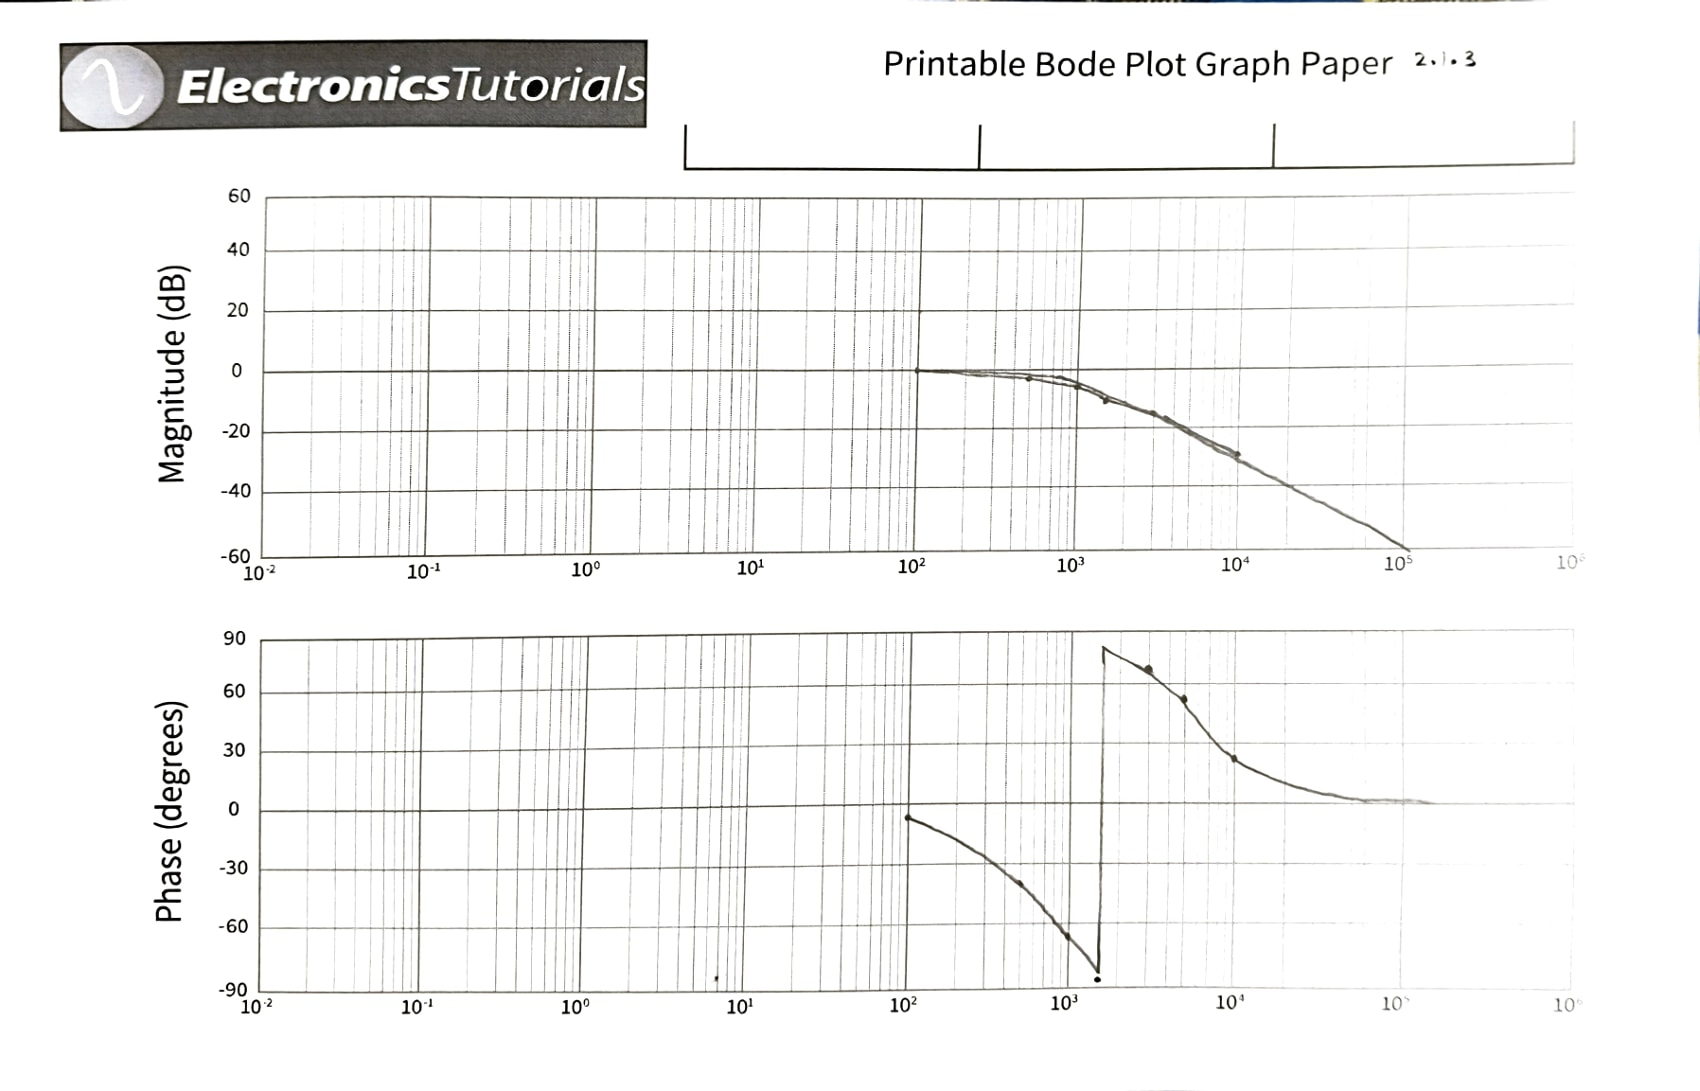
\includegraphics[width=\linewidth]{figs/2draw.jpg}
    
    \label{fig:enter-label}
\end{figure}
At low frequencies, the output approximates the input signal. As frequency increases, the magnitude decreases at a rate of \(-40\) dB/decade beyond the cutoff frequency \( f_c = \frac{1}{2\pi RC} \)


\chapter{Three-Stage RC Low-Pass Filter Setup}
\section{Three-Stage RC Low-Pass Filter Connection}
A three-stage RC low-pass filter provides even sharper roll-off characteristics, achieving \(-60\) dB/decade attenuation. This makes it highly effective for applications requiring significant noise suppression. Set up the connections as shown 

\subsection{Circuit Diagram}
\begin{figure}[H]
    \centering
    \begin{circuitikz}
        \draw
        (0,0) to[sV, v=$V_{in}$] (0,2)
        to[R, l=$R$] (2,2)
        to[C, l=$C$] (2,0)
        -- (0,0);
        \draw (2,2) to[R, l=$R$] (4,2)
        to[C, l=$C$] (4,0)
        -- (2,0);
        \draw (4,2) to[R, l=$R$] (6,2)
        to[C, l=$C$] (6,0)
        -- (4,0);
        \draw (6,2) to[short, -*] (7,2);
        \draw (6,0) to[short, -*] (7,0);
        \node[right] at (7,1) {$V_{out}$};
    \end{circuitikz}
    \caption{Three-Stage RC Low-Pass Filter Circuit}
\end{figure}
\subsection{Theoritical equations}
The expected output voltage is given by:
\begin{align}
 H_3(\omega) &= \frac{1}{1  + 6 j\omega R C + 5(j\omega R C)^2+ (j\omega R C)^3}\\
 |H_3(\omega)| &= \frac{1}{\sqrt{(1 - 5(\omega R C)^2)^2 + (6\omega R C + (\omega R C)^3)^2}}\\
 \theta_3(\omega) &= -\tan^{-1} \left( \frac{6\omega R C + (\omega R C)^3}{1 - 5(\omega R C)^2}  \right)
\end{align}
The magnitude response in decibels (dB) is given by:

\begin{align}
20 \log_{10} |H(\omega)|
\end{align}
The phase response in degrees is:

\begin{align}
\theta(\omega) \times \frac{180}{\pi}
\end{align}

where \( H(j\omega) \) is the transfer function.
\section*{3-Stage RC Low-Pass Filter Analysis}
\begin{table}[h]
    \centering
    \begin{tabular}{r c c c c}
        \toprule
        $f$(Hz) & $V_{in}$(V) & $V_{out}$ Theoretical(V) & $V_{out}$ Experimental(V)& $\Delta t$ \\
        \midrule
        100  & 2.161 & 2.058 & 1.982 & -595.621$\mu s$ \\
        500  & 2.161 & 1.124 & 1.041 & -426.354$\mu s$\\
        1000 & 2.161 & 0.591 & 0.601 & 215.716$\mu s$\\
        1590 & 2.161 & 0.338 & 0.312 & 108.669$\mu s$\\
        3000 & 2.161 & 0.124 & 0.139 & 45.076$\mu s$ \\
        5000 & 2.161 & 0.043 & 0.056 & 26.123$\mu s$\\
        10000 & 2.161 & 0.008 & 0.015 & 16.787$\mu s$ \\
        \bottomrule
    \end{tabular}
    \caption{3-Stage RC Low-Pass Filter Analysis}
\end{table}
\begin{itemize}
    \item The values of $\Delta t$ are taken by measuring difference between peaks.
    \item The signs of $\Delta t$ were placed according to the theory for correct phase plot.
\end{itemize}
\subsection{Bode Plot}
\begin{figure}[H] % H forces the figure to be placed exactly here
    \centering
    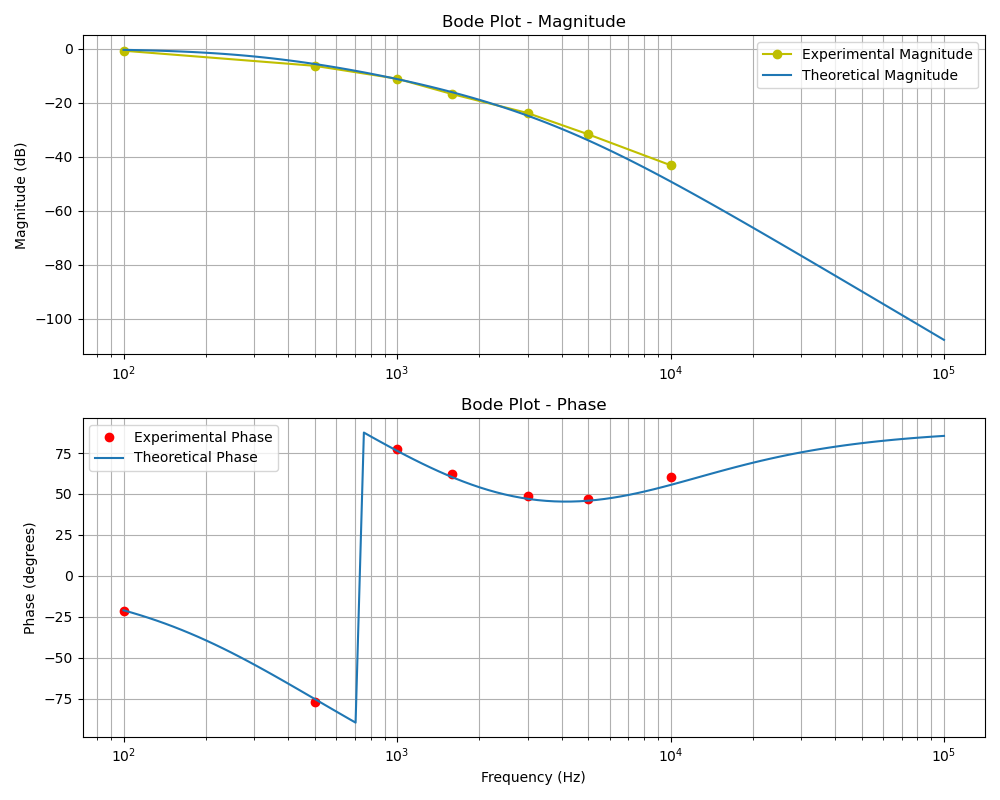
\includegraphics[width=\textwidth]{figs/3phase.png} % Replace "1.jpg" with your actual image filename
    
    \caption{3 stage bode plot}
    \label{fig:bode plot}
\end{figure}
\begin{figure}
    \centering
    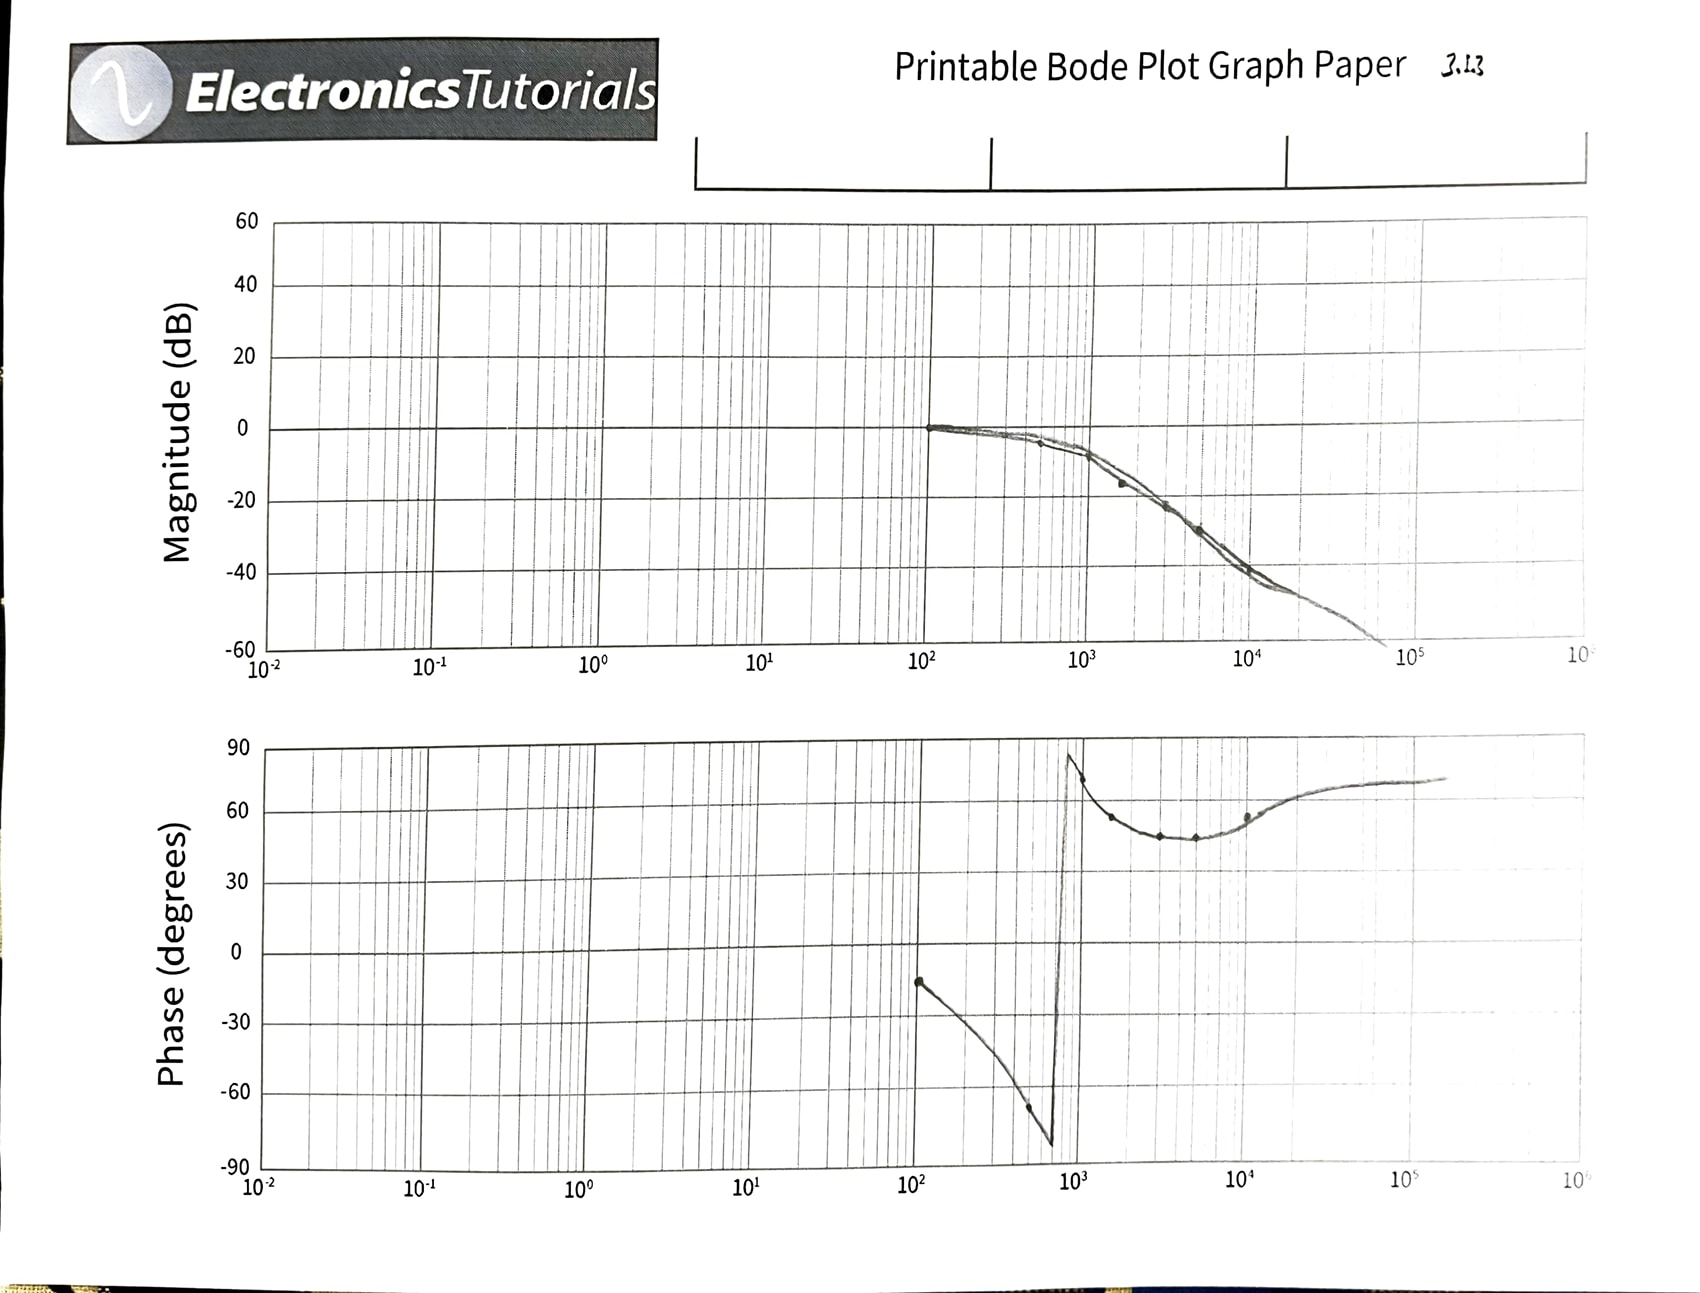
\includegraphics[width=\linewidth]{figs/3draw.jpg}
    
    \label{fig:enter-label}
\end{figure}



\end{document}
